\documentclass[10pt]{beamer}
\usepackage{ctex, hyperref}
\usepackage[T1]{fontenc}

\usepackage[backend=bibtex, sorting=none]{biblatex}
\addbibresource{ref.bib}
\setbeamertemplate{bibliography item}[text]
\setbeamerfont{footnote}{size=\tiny}

% other packages
\usepackage{latexsym,amsmath,xcolor,multicol,booktabs,calligra}
\usepackage{graphicx,pstricks,listings,stackengine}
 \usepackage{indentfirst}

\author{徐麦 \and 刘创}
\title{基于网约车轨迹数据的路网拥堵识别及预测}
\subtitle{第40期PRP结题答辩}
\institute{上海交通大学密西根学院 \newline \newline 指导老师: 高林杰}
\date{2022年3月9日}
\usepackage{SJTU}

% defs
\def\cmd#1{\texttt{\color{red}\footnotesize $\backslash$#1}}
\def\env#1{\texttt{\color{blue}\footnotesize #1}}
\definecolor{deepblue}{rgb}{0,0,0.5}
\definecolor{deepred}{rgb}{0.6,0,0}
\definecolor{deepgreen}{rgb}{0,0.5,0}
\definecolor{halfgray}{gray}{0.55}

\lstset{
    basicstyle=\ttfamily\footnotesize,
    keywordstyle=\bfseries\color{deepblue},
    emphstyle=\ttfamily\color{deepred},    % Custom highlighting style
    stringstyle=\color{deepgreen},
    numbers=left,
    numberstyle=\small\color{halfgray},
    rulesepcolor=\color{red!20!green!20!blue!20},
    frame=shadowbox,
}


\begin{document}
\heiti
\begin{frame}
    \titlepage
    \begin{figure}[htpb]
        \begin{center}
            
\includegraphics[width=0.18\linewidth]{pic/SJTU.png}
        \end{center}
    \end{figure}
\end{frame}

\begin{frame}
    \tableofcontents[sectionstyle=show,subsectionstyle=show/shaded/hide,subsubsectionstyle=show/shaded/hide]
\end{frame}


\section{研究背景与意义}

\begin{frame}{背景}
\begin{figure}
\centering
\begin{minipage}[t]{0.48\textwidth}
\centering
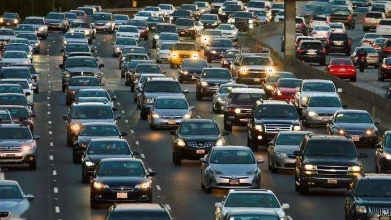
\includegraphics[width=5cm]{pic/1.png}
\caption{堵车现象}
\end{minipage}
\begin{minipage}[t]{0.48\textwidth}
\centering
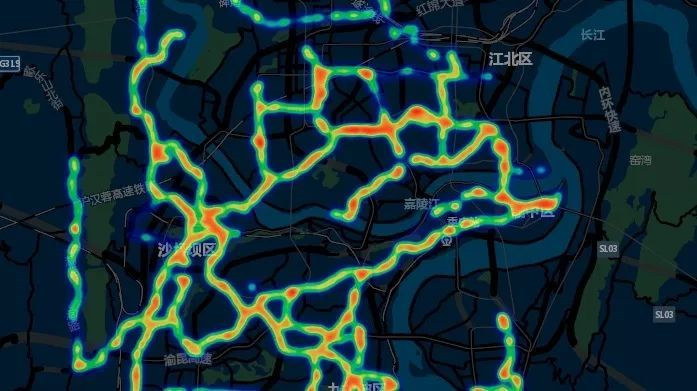
\includegraphics[width=5cm]{pic/2.png}
\caption{车辆轨迹数据可视化}
\end{minipage}
\end{figure}
\par 随着城市和城际交通压力增大,面对海量交通轨迹数据,人们愈加需要\alert{研究并分析数据特征},对于堵车现象建立相应\alert{模型预测识别}。
\\ \hspace*{\fill} \\
\par 关键词:\color{blue} 轨迹大数据,深度学习(神经网络),预测模型。
\end{frame}

\section{研究内容与方法}

\begin{frame}{研究流程}
    \begin{figure}
        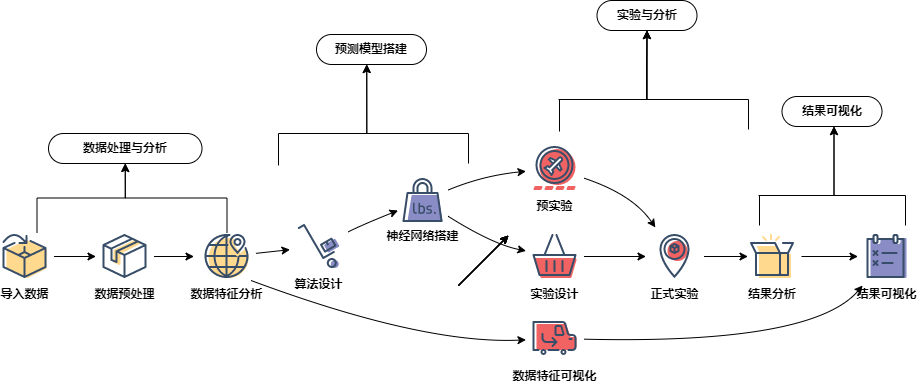
\includegraphics[width=9.9cm]{pic/研究流程图.png}
        \caption{研究流程}
        \label{fig.chart}
    \end{figure}
\end{frame}

\begin{frame}{研究范围}
\par 研究区域 —— 成都市市中心
   \begin{figure}[htb] 
        \centering
        \begin{minipage}[b]{0.4\textwidth} 
        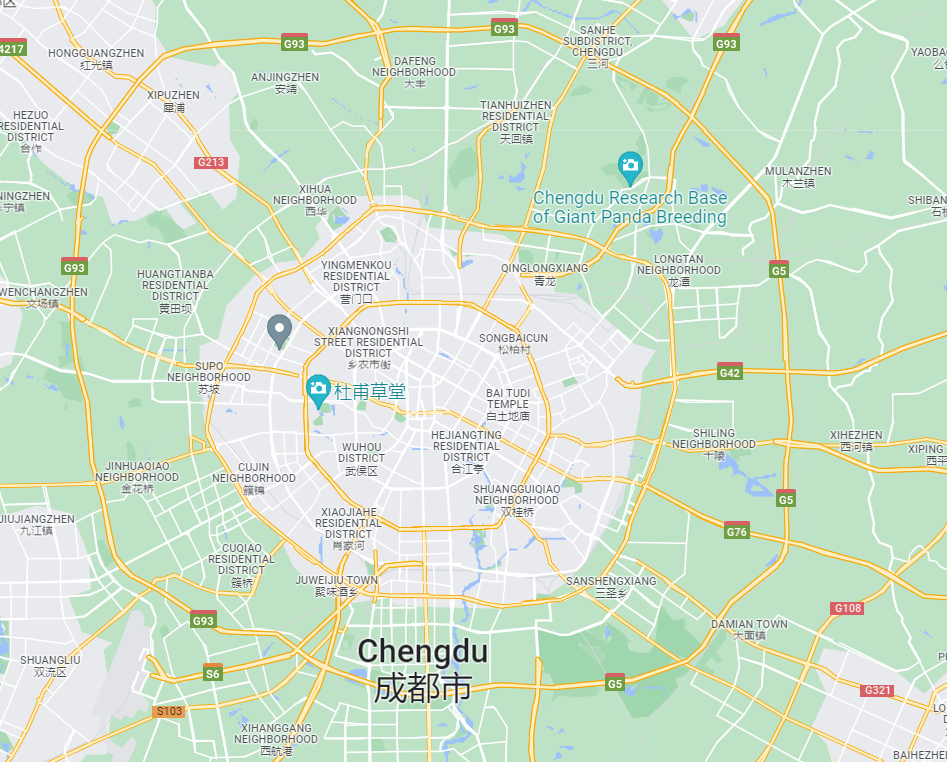
\includegraphics[width=0.8\textwidth]{pic/map.png} 
        \caption{成都市市中心概况} 
        \label{fig.map} 
        \end{minipage}% 
        \begin{minipage}[b]{0.6\textwidth} 
        \footnotesize
        \centering
        \begin{tabular}{|c|c|} \hline 
        网约车司机ID & opqlvh8hc1yjyh6iCBooqrkhdmi_stBe \\ \hline
        订单ID    & jjylseig5_zoyi_rrrndqzyndmd1zpwl  \\ \hline
        Unix时间戳   & 1477969147 \\ \hline
        经度 & 104.07513 \\ \hline
        纬度  & 30.72724 \\ \hline 
        \end{tabular} 
        \caption{原始数据样例} 
        \label{table:by:fig} 
        \end{minipage} 
    \end{figure} 
\par 数据概况:
\begin{itemize}
        \item 呈现很好的\alert{结构性}
        \item 包含了详细经纬度信息和时间序列信息,能够从中提取\alert{时空特征信息}
        \item 个别部分呈现\alert{缺失值}仍需要预处理
\end{itemize}
\end{frame}

\section{研究过程与结果分析}
\subsection{数据预处理与分析}
\begin{frame}{预处理步骤}
    \begin{figure}
        \centering
        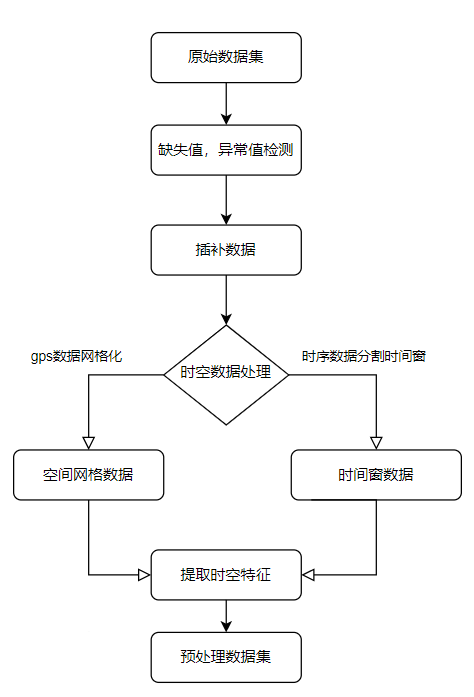
\includegraphics[width=4cm]{pic/流程图.png}
        \caption{流程图}
        \label{fig.workflow}
    \end{figure}
\end{frame}

\begin{frame}{数据特征分析:周期性}
    \begin{figure}
        \centering
        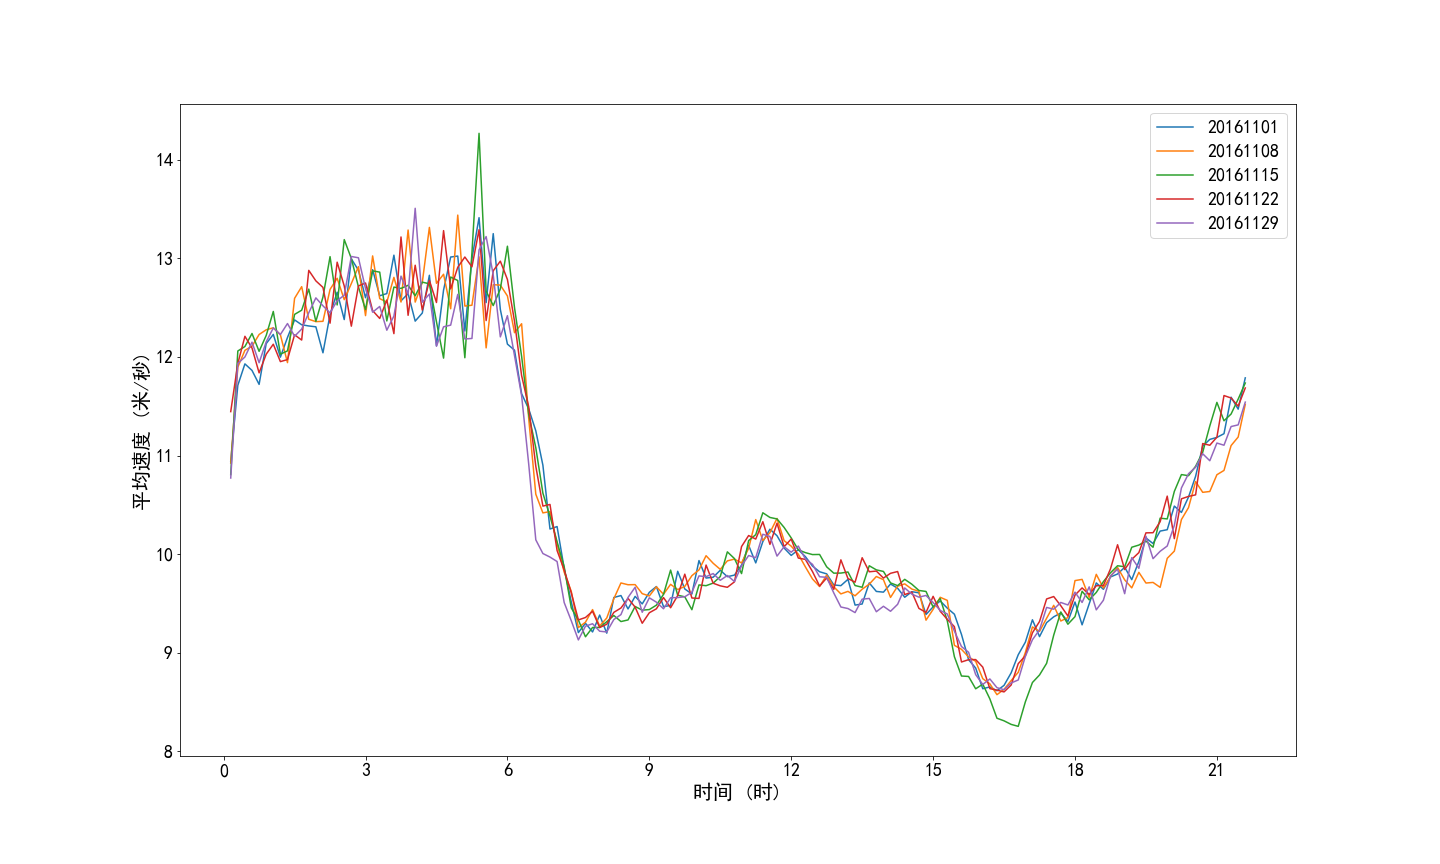
\includegraphics[width=8cm]{pic/五个周二平均速度线型图.png}
        \caption{2016年11月每周周二网格平均速度趋势图}
        \label{fig.period}
    \end{figure}
    \begin{itemize}
        \item 每周每天相同时间的平均速度趋势相似,呈现\alert{周期性}。
        \item 相邻几天相同时间的平均速度趋势相似,呈现\alert{邻域连贯性\footfullcite{PCNN}}。
        \item 平均车速折线两端\alert{局部最低}分别对应\alert{早晚高峰}(7-9;16-18)。
\end{itemize}
\end{frame}

\begin{frame}{数据特征分析:邻域连贯性}
    \par 将预处理后数据后得到的\alert{网格平均速度值},呈现出\alert{邻域连贯性}:
    \\ \hspace*{\fill} \\
    \par 根据Chen的研究\footfullcite{PCNN},一个交通网格在某一时刻的网格速度与其在空间和时间上邻近的网格的差距在一定的距离范围内可视为是连贯的。这是因为大部分时间段的交通状况很少出现突变的情况。
    \\ \hspace*{\fill} \\
    \par 因此我们认为,同时考虑\alert{一定时空邻域内的所有数据}对于预测某个时空网格的数据是有帮助的。
\end{frame}

% ------------------------------ %
\subsection{算法设计}

\begin{frame}{卷积神经网络}

    \begin{block}{简介}
       卷积神经网络(Convolutional Neural Network, CNN)是深度学习领域最具代表性的算法之一。其核心思路是通过卷积运算和深层的网络结构,高效地捕捉高维数据中的\alert{隐藏特征},并完成分类和\alert{回归}任务。
    \end{block}
    
    \begin{block}{算法适用性}
        \begin{itemize}
            \item 整个交通网络在同一时刻的数据可以视为一个由横纵坐标编码的\alert{二维速度矩阵}。而不同时刻的数据间存在\alert{邻域相关性}和\alert{周期性}。
            \item 将间隔一定时间的数据矩阵叠加在一起,从多个通道一起输入神经网络,从而尝试让模型记忆并预测出交通拥堵的邻域相关性和周期性特征,最终提高预测性能。
        \end{itemize}
    \end{block}
    
\end{frame}

% ------------------------------ %
\subsection{神经网络设计}

\begin{frame}{输入层}
    \begin{block}{设计}
       考虑到交通数据的邻域连贯性和周期性,我们采用\alert{数据裁剪}来结合各个网格与它们空间上的邻域的数据;同时,每一个时刻的速度矩阵都会和与它在时间上相邻的速度矩阵从\alert{多个通道}同时送入CNN进行处理,从而使CNN捕捉到数据在时空上的连贯性和周期性。
    \end{block}
    
    \begin{block}{数据裁剪}
        \begin{itemize}
            \item 目的:使CNN捕捉到数据在\alert{空间上的相关性};扩大训练数据量
        \end{itemize}
    \end{block}
    
    \begin{block}{多通道输入}
    \begin{itemize}
        \item 输入张量的结构可分为\alert{标签层}和\alert{数据层}。
        \item 标签层:待预测时刻$m$的速度网格。
        \item 数据层:过去$t$小时中加上过去$d$天中,同一时刻的网格速度。
        \item 目的:使CNN捕捉到数据在时空上的\alert{连贯性}和\alert{周期性}。
    \end{itemize}
    \end{block}
\end{frame}



\begin{frame}{神经网络搭建}
    \begin{block}{隐藏层结构}
    隐藏层参考由LeCun\footfullcite{lecun1998gradient}设计的\alert{“卷积-池化”结构}。特别地,考虑到卷积和池化操作可能会使特征图的尺寸缩小,我们选择在最后一个卷积层前增加一个\alert{上采样层}来恢复特征图的尺寸
    \end{block}
    
    \begin{block}{优化算法与目标函数}
        \begin{itemize}
            \item 优化策略:Adam优化器
            \item 目标函数:均方误差(MSE)\\
            \begin{equation}
                \frac{1}{n} \sum_{i=1}^{n} \left( Y_i - \hat{Y_i} \right)^2
            \end{equation}
            \end{itemize}
    \end{block} 
\end{frame}
% ------------------------------ %
\subsection{实验设计}

\begin{frame}{性能评价标准}
    本研究中,我们综合四个性能指标来评价模型的回归性能:
     \begin{itemize}
         \item MSE: $\frac{1}{n} \sum_{i=1}^{n} \left( Y_i - \hat{Y_i} \right)^2$
         \item RMSE:  $ \sqrt{\frac{1}{n} \sum_{i=1}^{n} \left( Y_i - \hat{Y_i} \right)^2}$
         \item MAE: $\frac{1}{n} \sum_{i=1}^{n} \left| Y_i - \hat{Y_i} \right|$
         \item $R^2$: $1 - \frac{\sum_{i=1}^{n} (y_i - \hat{y_i})^2}{\sum_{i=1}^{n} (y_i - \bar{y_i})^2}$
         
     \end{itemize}
\end{frame}

\subsection{预实验}
\begin{frame}{实验目的}
    为了尽量提高CNN性能,需要为神经网络找到合适的超参数,在本研究中包括\alert{输入张量的形状}、\alert{优化器学习率}以及训练的\alert{批尺寸}。因此,在正式实验之前,我们选择用11月1日到5日的数据进行预实验,即用前四天的数据训练模型,以目标函数作为误差,预测第五天的数据。
\end{frame}

\begin{frame}{输入张量的形状}
    将输入张量的形状$t$与$d$作为变量,实验结果如图\ref{fig.inputShape}所示。当\alert{$t=2, d=2$}时,误差达到最低。
    \begin{figure}
        \centering
        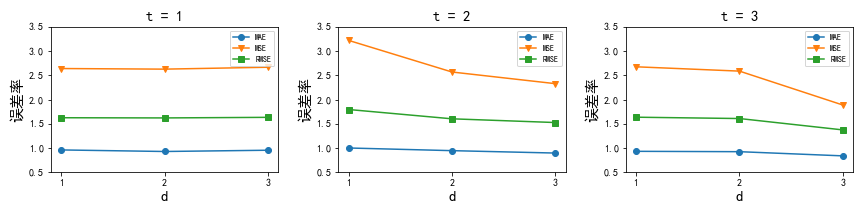
\includegraphics[width=11cm]{pic/combine.png}
        \caption{对输入张量实验的预实验结果}
        \label{fig.inputShape}
    \end{figure}
\end{frame}

\begin{frame}{学习率}
    将优化器的学习率作为变量,实验结果如图\ref{fig.learningRate}所示。当学习率为\alert{$0.0002$}时,误差达到最低。
    \begin{figure}
        \centering
        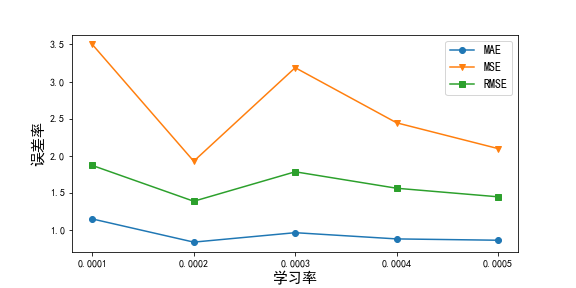
\includegraphics[width=10cm]{pic/lr.png}
        \caption{对学习率的预实验结果}
        \label{fig.learningRate}
    \end{figure}
\end{frame}

\begin{frame}{批尺寸}
    将批尺寸作为变量,实验结果如图\ref{fig.batchSize}所示。在批尺寸为\alert{$32$}时,误差达到最低。
    \begin{figure}
        \centering
        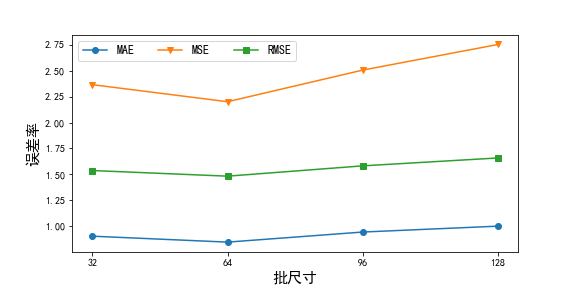
\includegraphics[width=10cm]{pic/bs.png}
        \caption{对批尺寸的预实验结果}
        \label{fig.batchSize}
    \end{figure}
\end{frame}

\subsection{正式实验}
\begin{frame}{实验内容}
    \begin{block}{实验目的}
       用CNN处理已经预处理后的数据集,用前29天的数据预测第30的全部网格速度数据。
    \end{block}
    \begin{block}{实验设计}
       网络输入层和隐藏层结构如图\ref{tab.CNNstructure}所示。Adam优化器的学习率为0.0002,训练批尺寸为64.前29天的速度数据在重整为特定形状的张量以后输入模型进行训练。最后,用训练所得的模型预测第30天的数据。
       \begin{figure}
           \centering
           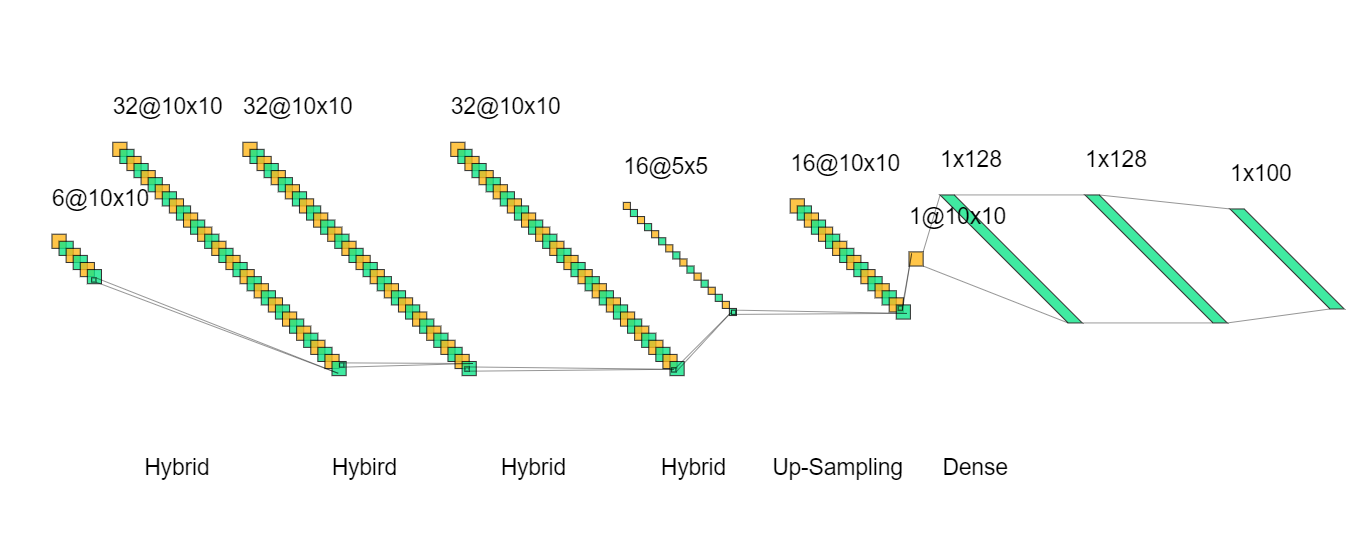
\includegraphics[width=8cm]{pic/cnn.png}
           \caption{CNN结构}
           \label{tab.CNNstructure}
       \end{figure}
    \end{block}
\end{frame}

\subsection{实验结果}
\begin{frame}{模型性能}
    对第30天数据预测的整体误差在表\ref{tab.finalPerformance}中给出。其中\alert{决定系数达到0.89},表明模型表现出较好的回归性能。
    \begin{table}[h!]
        \centering
        \begin{tabular}{|c|c|c|c|}
        \hline
            MAE & MSE & RMSE & $R^2$ \\
            \hline
            0.617 & 1.068 & 1.034 & 0.893 \\
            \hline
        \end{tabular}
        \caption{最终模型性能参数}
        \label{tab.finalPerformance}
    \end{table}
\end{frame}

\begin{frame}{结果可视化}
    图\ref{tab.lineGraph}为所研究路网中的其中6个网格的平均速度的预测值和真实值。
    \begin{itemize}
        \item 模型对于平均速度的\alert{总体趋势}的预测较为准确。
        \item 不擅于预测\alert{短时间范围内出现的速度突变}。
    \end{itemize}
    
    \begin{figure}
        \centering
        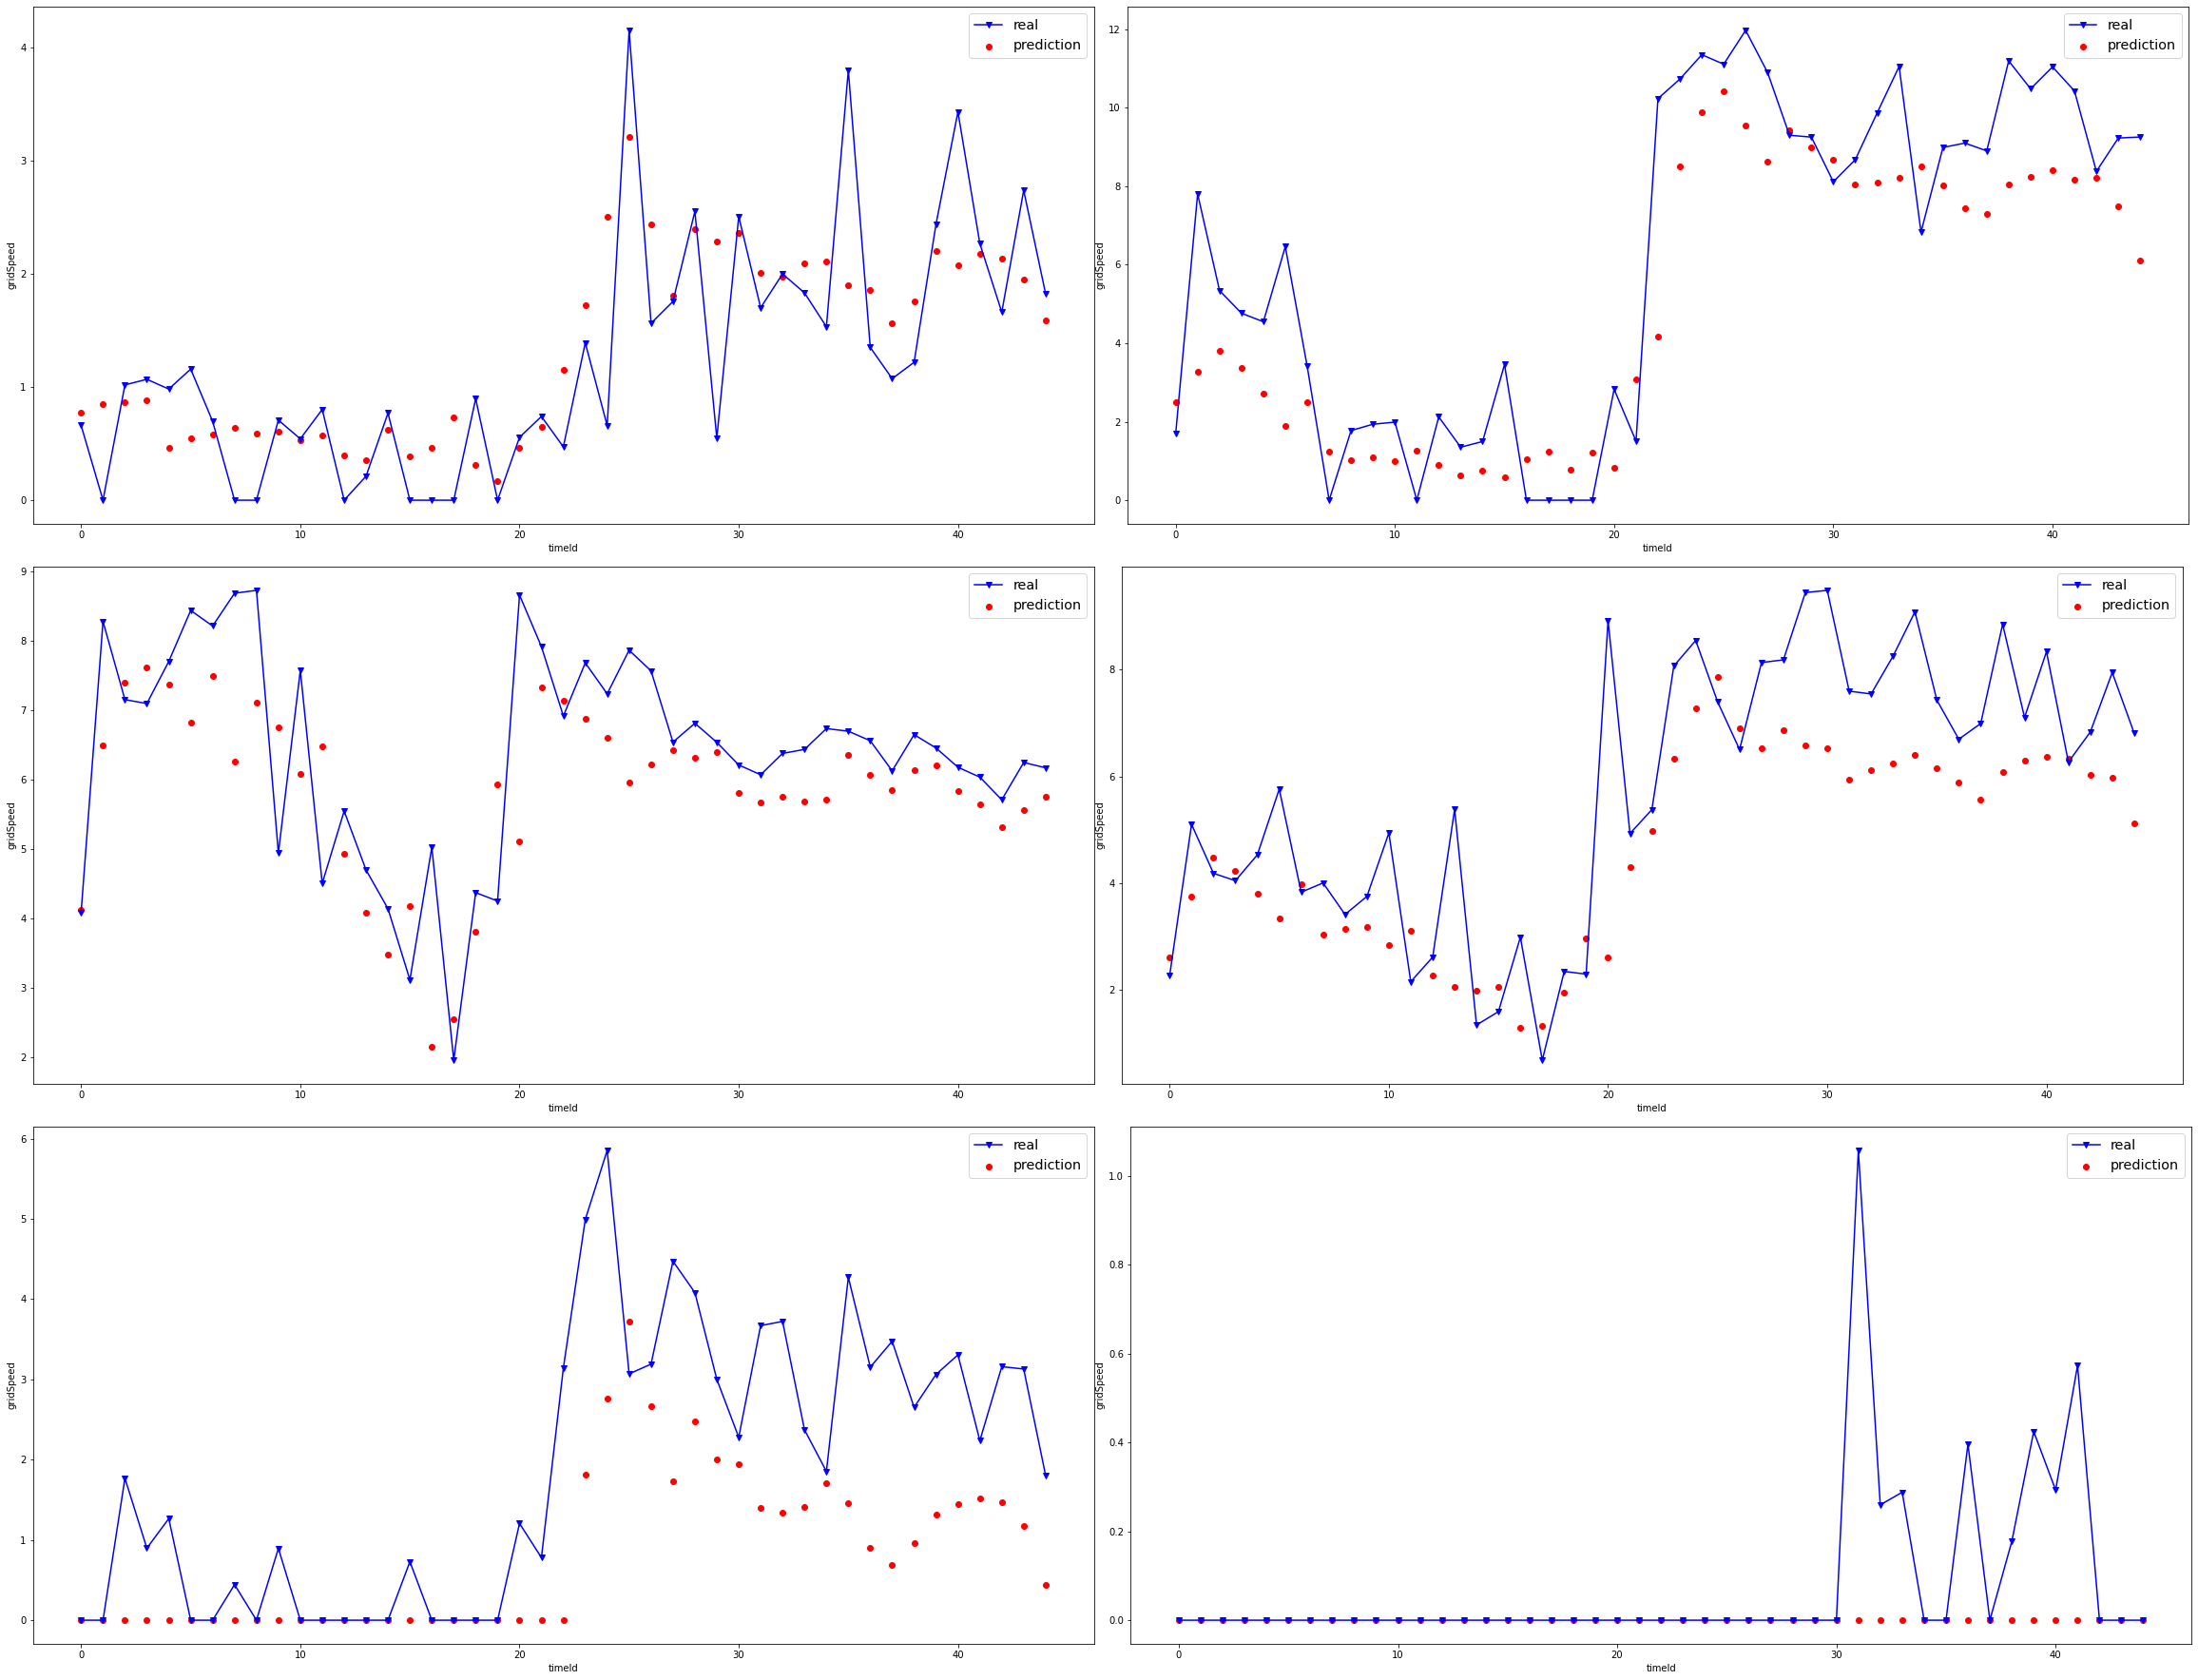
\includegraphics[width=6cm]{pic/3x2.png}
        \caption{预测结果折线图}
        \label{tab.lineGraph}
    \end{figure}
\end{frame}

\begin{frame}{结果可视化}
    图\ref{fig.heatmap}展示了网格预测与真实情况的热力图
    \begin{figure}
        \centering
        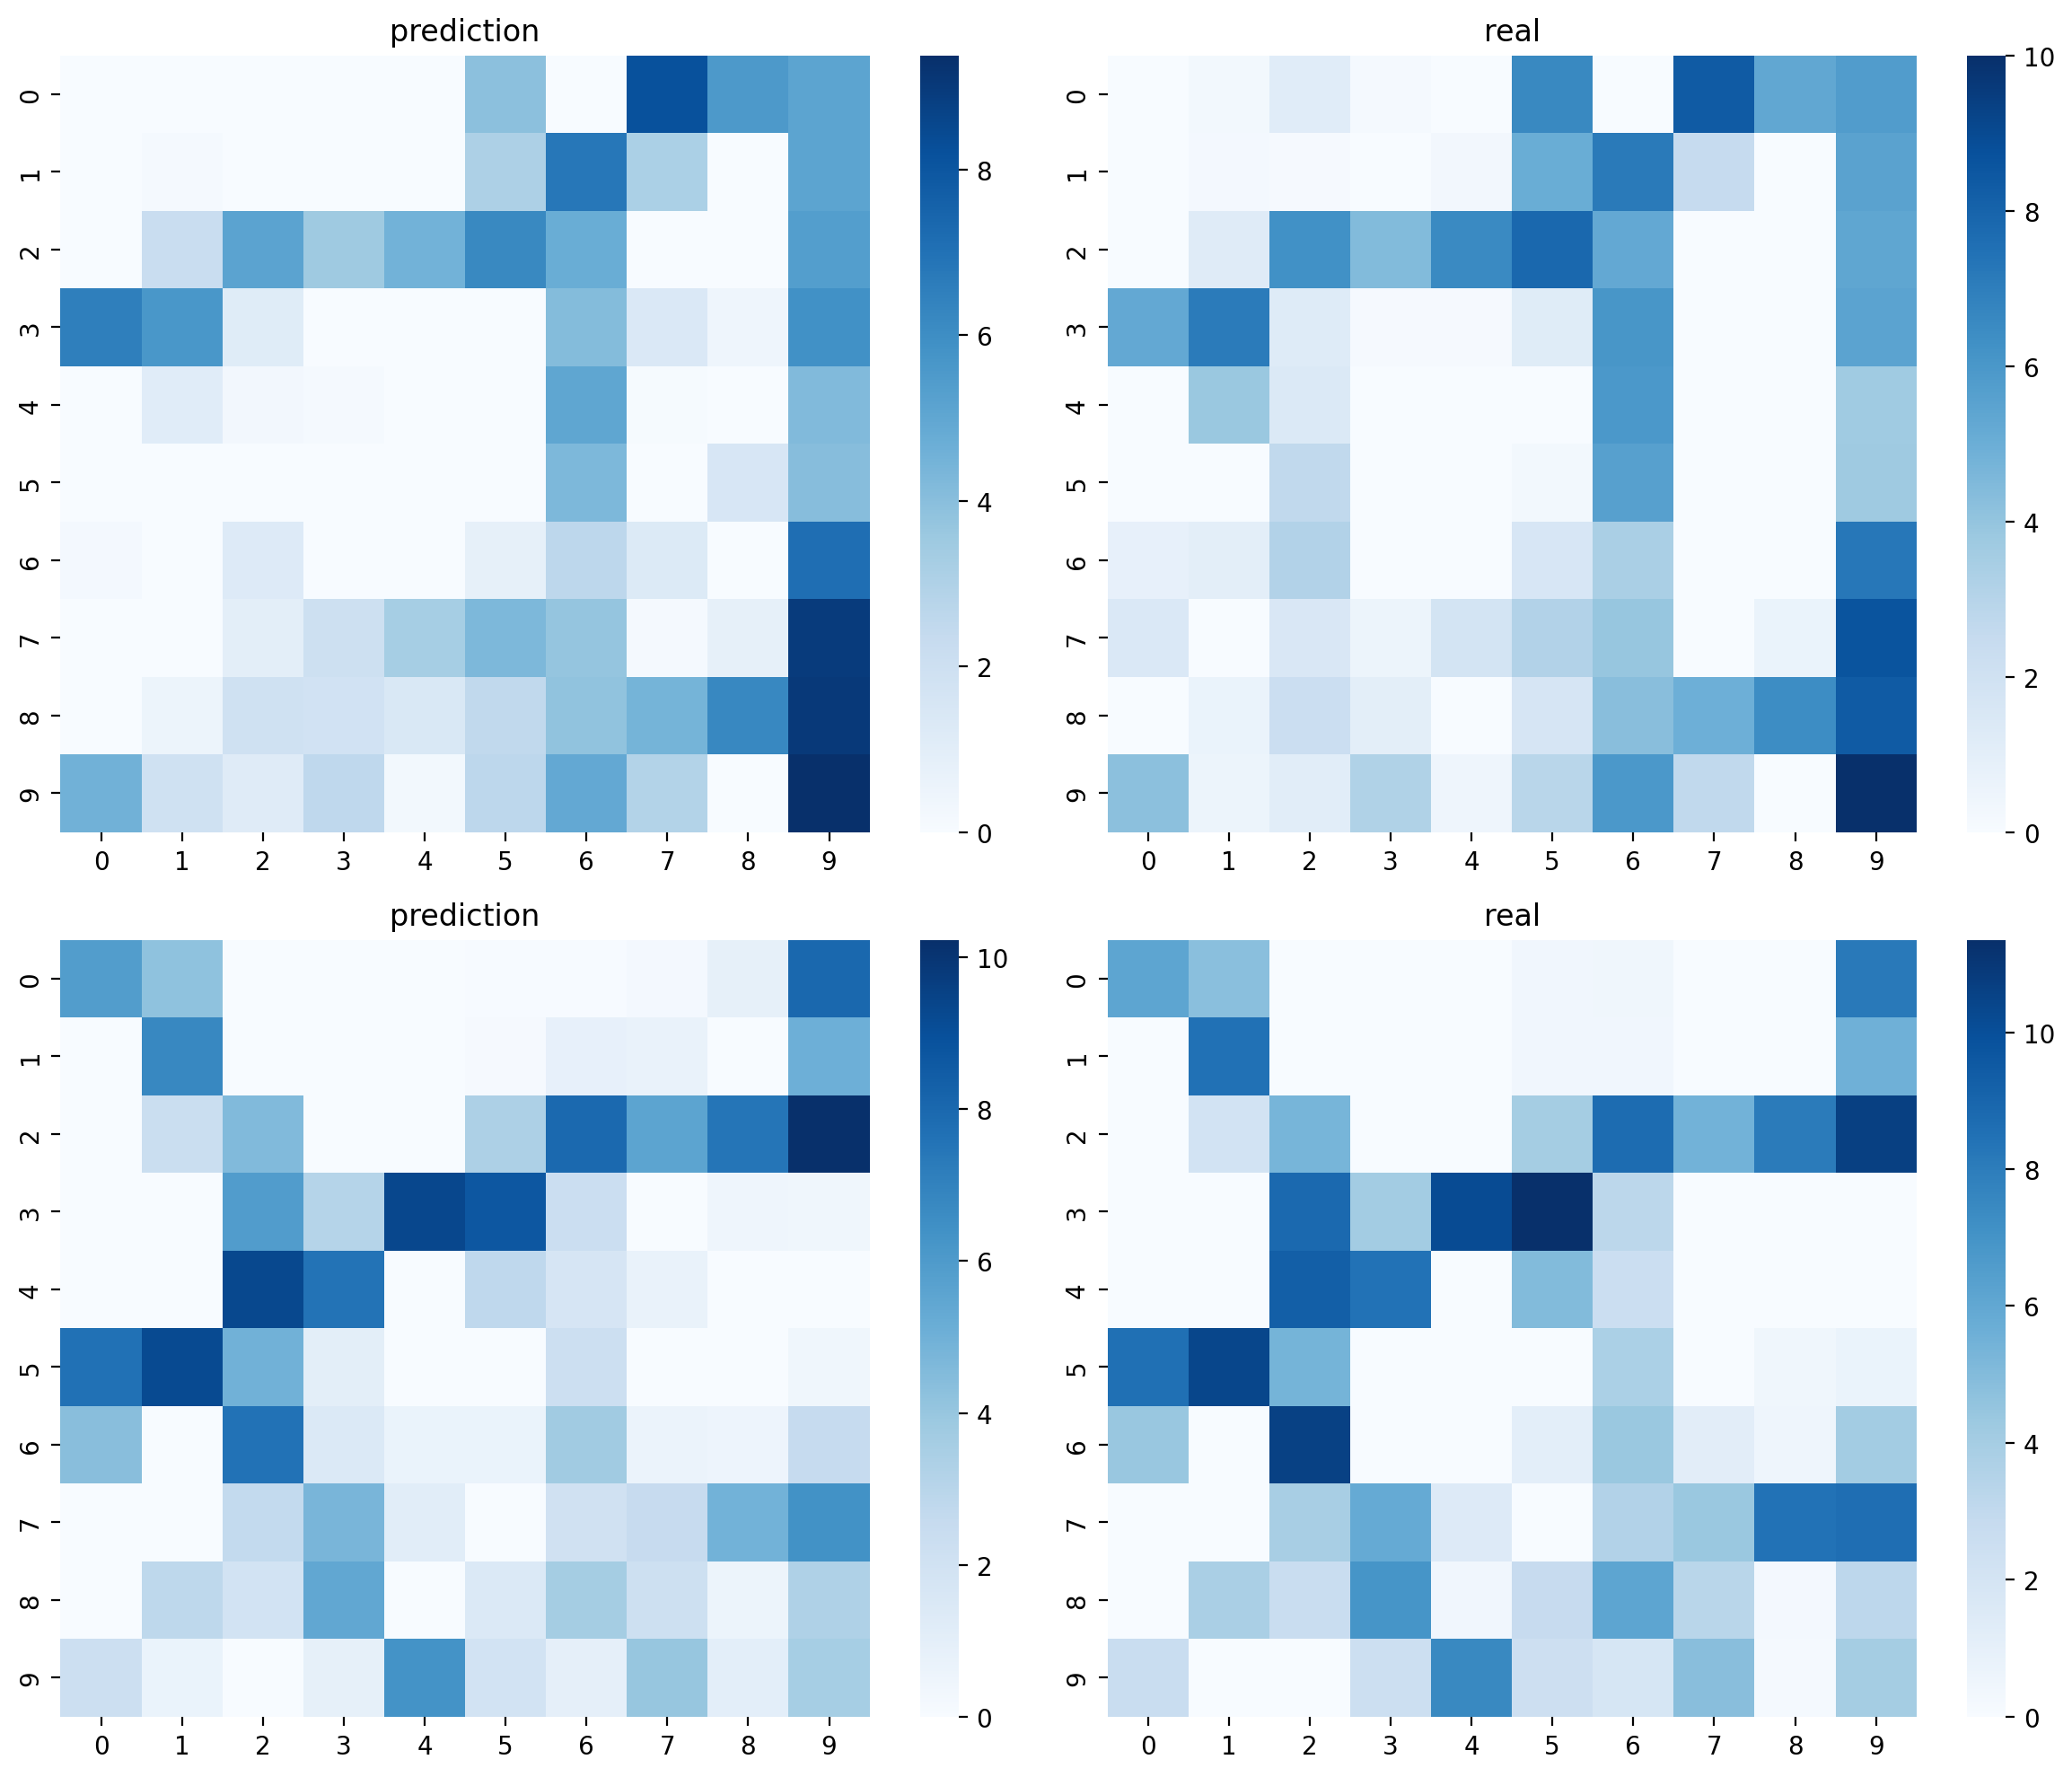
\includegraphics[width=7cm]{pic/output.png}
        \caption{预测结果热力图}
        \label{fig.heatmap}
    \end{figure}
\end{frame}


% ------------------------------ %
\subsection{结论}

\begin{frame}{研究结论}
    \begin{itemize}
        \item 在本研究中,我们提出了一种用于预测短期交通拥堵状况的深度学习算法。整个算法基于卷积神经网络。考虑到交通数据往往具有连贯性和周期性,我们在输入层的选择和网络结构上做出了一定创新,将隔日与隔小时的数据相结合同时作为输入。
        \item 实验结果表明,模型对于一整日交通速度变化信息的预测表现出了\alert{较强的回归性能}。这说明该算法设计可以用于交通拥堵状况的预测,从而辅助交通管理决策。
    \end{itemize}
\end{frame}

\section{总结展望}
\begin{frame}{算法优点}
    \begin{block}{优点总结}
       \begin{itemize}
            \item 训练时间短
            \item 实现了大范围的路网速度预测
            \item 预测精度较高
        \end{itemize} 
    \end{block}
    
    \begin{block}{横向对比}
       如表\ref{tab.comparison}所示,与一些传统的交通预测算法\footfullcite{bogaerts2020graph}进行对比,本算法在预测性能方面取得了一定的提升。
       \begin{table}[h!]
           \centering
           \begin{tabular}{|c|c|c|}
               \hline
               模型 & MAE & RMSE \\
               \hline
               k-NN & 1.388 & 3.065 \\
               \hline
               LSTM & 1.231 & 2.720 \\
               \hline
               SVM & 1.345 & 2.286 \\
               \hline
               本模型 & 0.526 & 0.883 \\
               \hline
           \end{tabular}
           \caption{与传统交通拥堵算法的性能对比}
           \label{tab.comparison}
       \end{table}
    \end{block}
\end{frame}

\begin{frame}{不足与应用前景}
    
    \begin{block}{不足}
          \begin{itemize}
            \item 基于网格化路段,忽略了\alert{路段的形状信息}
            \item 训练数据\alert{完全基于网约车},无法提取更多路段车流信息
            \item 由于数据集的时间跨度较小以及网格化,模型\alert{对突变数据的预测能力较差}
            \item 没有考虑\alert{更多影响交通的因素},如天气、节假日等
        \end{itemize}
    \end{block}
    
    \begin{block}{应用前景}
        本研究所提出的算法的预测值与真实值的误差相对较小,能够较好地预测网格车辆平均速度。而且模型能够实现\alert{同时对城市中心大片区域进行预测},对\alert{相对复杂、数量庞大}的城市道路交通流量进行预测是一种行之有效的手段。      
    \end{block}

\end{frame}

% ----------------------------- %
\section{参考文献}

\begin{frame}[allowframebreaks]{参考文献}
    \printbibliography
    % 如果参考文献太多的话,可以像下面这样调整字体:
    % \tiny\bibliographystyle{alpha}
\end{frame}

\begin{frame}
    \begin{center}
        {\Huge\calligra Thanks!}
    \end{center}
\end{frame}

\end{document}
